\documentclass[spanish,notes=hide,16pt]{beamer}

%To create 'handout' version (Copyright: Diego Berrueta)
%\documentclass[handout,notes=show]{beamer}

\usetheme{Marburg}
%\usepackage{beamerthemesplit}

\usepackage[spanish]{babel}
\usepackage[utf8]{inputenc}
\usepackage{listings}
\usepackage{graphicx}
\usepackage{colortbl}
\usepackage{array}
\usepackage{eurosym}

\title{Mailing lists meet the Semantic Web}
\author{
Sergio Fern\'andez\inst{1} 
\and
\textbf{Diego Berrueta}\inst{1} 
\and
Jose E. Labra\inst{2}
}
\institute{%
Fundaci\'on CTIC, \\
Gij\'on, Asturias, Spain,\\
\email{\{sergio.fernandez,diego.berrueta\}@fundacionctic.org}
\and
Universidad de Oviedo,\\
Computer Science Department,\\
Oviedo, Asturias, Spain,\\
\email{labra@uniovi.es}\\
}
\date{27 April 2007}

\begin{document}


%tableofcontents

%\AtBeginSection[]
%{
%   \begin{frame}
%       \frametitle{Tabla de contenidos}
%       \tableofcontents[currentsection]
%   \end{frame}
%}

%\AtBeginSubsection[] 
%{
%   \begin{frame}
%       \frametitle{Tabla de contenidos}
%       \tableofcontents[currentsection,currentsubsection]
%   \end{frame}
%}

%listings

\definecolor{darkred}{rgb}{0.5, 0, 0}
\definecolor{violet}{rgb}{1, 0, 1}
\definecolor{green}{rgb}{0.3, 0.95, 0.3}
\definecolor{listinggray}{gray}{0.97}

\lstset{
	basewidth=0.50em,
	backgroundcolor=\color{listinggray},
	basicstyle=\footnotesize\ttfamily,
	keywordstyle=\bfseries,
	stringstyle=\itshape,
	commentstyle=\itshape,
	showspaces=false,
	showtabs=false,
	showstringspaces=false,
	frame=trbl,
	extendedchars=true,
	numbers=none,
	aboveskip=0.5cm,
	belowskip=0.5cm,
	xleftmargin=0cm,
	xrightmargin=0cm
}

\lstdefinelanguage{mbox}{%no funciona!
	morekeywords = {From, Message, Date, Organization, To, Subject }
}

\lstdefinelanguage{SPARQL}{%
	morekeywords = {PREFIX, SELECT, DISTINCT, WHERE }
}

\defverbatim[colored]\MBOX{
\lstset{language=mbox}
\begin{lstlisting}
...
From sioc-dev@googlegroups.com Fri Sep 15 13:35:44 2006
Message-ID: <1158352519.450b0e871c79e@courrier.privatedns.com>
Date: Fri, 15 Sep 2006 16:35:19 -0400
From: Frederick Giasson <fred@fgiasson.com>
To: sioc-dev@googlegroups.com
Subject: Implementation of the SIOC v1.08 ontology in Talk Digger
...
From sioc-dev@googlegroups.com Tue Sep 19 07:10:22 2006
From: Kjetil Kjernsmo <kjetilk@opera.com>
Organization: Opera Software ASA
To: sioc-dev@googlegroups.com
Subject: Re: User vs. Person complexity
Date: Tue, 19 Sep 2006 16:09:15 +0200
...
\end{lstlisting}
}

\defverbatim[colored]\SPARQL{
\lstset{language=SPARQL}
\begin{lstlisting}
PREFIX foaf: <http://xmlns.com/foaf/0.1/>

FROM <http://www.wikier.org/foaf.rdf>

SELECT ?nick, ?name

WHERE {
  ?x a foaf:Person .
  ?x foaf:nick ?nick .
  ?x foaf:name ?name
}
\end{lstlisting}
}


\maketitle

\section{Introduction}
\frame
{
  \frametitle{Introduction}

  \begin{itemize}
   \item<2-> \begin{large}\textbf{Current situation:}\end{large}
	\begin{itemize}
	  \item \begin{large}Thousands of mailing lists\end{large}
	  \item \begin{large}HTML (syntactic) publication\end{large}
	\end{itemize}
   \vspace{1cm}
   \item<3-> \textbf{Problems:}
	\begin{itemize}
	  \item \begin{large}Loss of information\end{large}
	  \item \begin{large}Structured markup without any semantic meaning\end{large}
	  \item \begin{large}Problems with traditional searches\end{large}
	\end{itemize}
  \end{itemize}
}

\section{The Semantic Web}
\frame
{
  \frametitle{The Semantic Web}

  \begin{Large}
    The semantic web is an evolving \textbf{extension} of the World Wide Web in 
    which web content can be expressed in a form that can be understood, 
    interpreted and used by machines.
  \end{Large}
  
  \vspace{1cm}

  \begin{Large}
    It derives from W3C director Tim Berners-Lee's vision of the Web as a universal 
    medium for \textbf{data}, \textbf{information} and \textbf{knowledge} exchange.
  \end{Large}
}
\frame
{
  \frametitle{Semantic Web stack}

  \begin{center}
    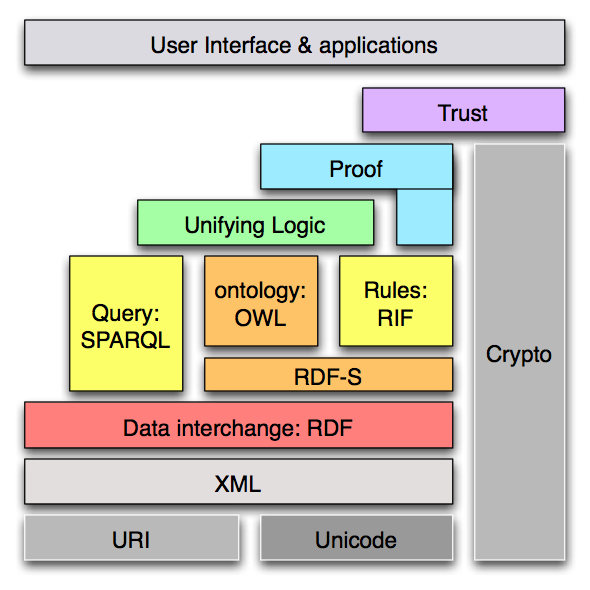
\includegraphics[width=0.8\textwidth]{images/semantic-web-stack.png}
  \end{center}

}
\frame
{
  \frametitle{RDF}

  \begin{Large}
     \textbf{R}esource \textbf{D}escription \textbf{F}ramework is a family W3C
     technologies to model information.
  \end{Large}

  \vspace{0.7cm}

  \begin{Large}
     RDF is based upon a triples metadata model:
     \begin{center}
       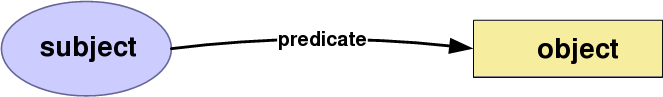
\includegraphics[width=0.8\textwidth]{images/triple.png}
     \end{center}
     The \textbf{subject} of an RDF statement is a resource, possibly as named by 
     a Uniform Resource Identifier (URI). The \textbf{predicate} is a resource as 
     well, representing a relationship. The \textbf{object} is a resource or a 
     Unicode string literal.
  \end{Large}
}

\section{SIOC}
\frame
{
  \frametitle{SIOC Ontology}

  \begin{Large}
    \textbf{S}emantically-\textbf{I}nterlinked \textbf{O}nline \textbf{C}ommunities 
    is an ontology that provides a vocabulary to interconnect different discussion 
    methods such as blogs, web-based forums and mailing lists.
  \end{Large}

  \begin{center}
    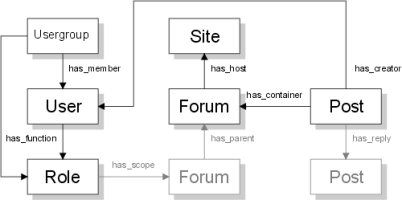
\includegraphics[width=0.8\textwidth]{images/sioc-terms.png}
  \end{center}


}
\frame{
  \frametitle{Extending SIOC Ontology}

  \begin{Large}
     SIOC is an almost perfect match for our purpose, using instances of
     \texttt{sioc:Forum}, \texttt{sioc:Post} and \texttt{sioc:User} classes.
  \end{Large}

  \vspace{0.7cm}

  \begin{Large}
    However, additional object properties were required in order to retain the 
    sequence of messages published in a mailing list. Thus, we extended the SIOC 
    ontology with \textbf{two new properties}.
  \end{Large}

}

\section{Software tools}
\frame
{
  \frametitle{Software tools}

  We built two software tools as part of this project:
  \vspace{0.5cm}
  \begin{itemize}
    \item<2->	\begin{Large}\textbf{SWAM}L is a non-interactive, 
		command-line application whose main purpose is to 
		translate mailboxes into sioc:Forum instances in 
		RDF.\end{Large}
    \vspace{0.5cm}
    \item<3->	\begin{Large}\textbf{Buxon} is a graphical browser 
		for \texttt{sioc:Forum} instances.\end{Large}
  \end{itemize}
}
\frame
{
  \frametitle{Software tools}

  \begin{center}
    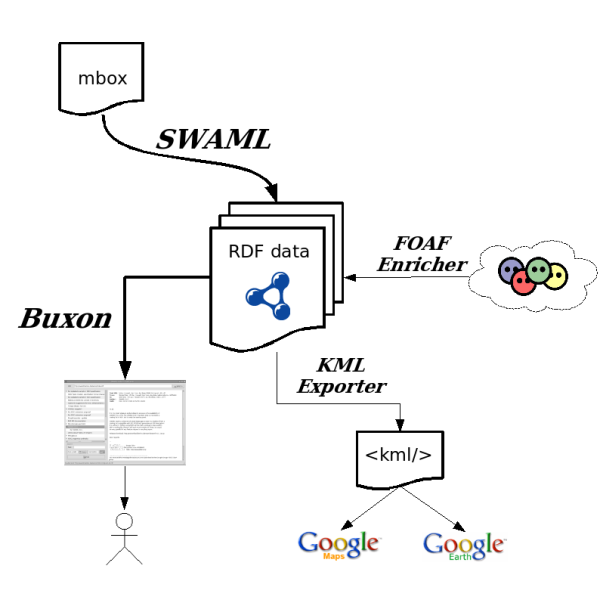
\includegraphics[width=0.85\textwidth]{images/swaml-tools.png}
  \end{center}
}
\frame
{
  \frametitle{SWAML}

  \begin{columns}
   \begin{column}{0.5\textwidth}
	\begin{center}
	  \only<1>{
\includegraphics[width=0.95\textwidth]{images/swaml-0.png}}
	  \only<2>{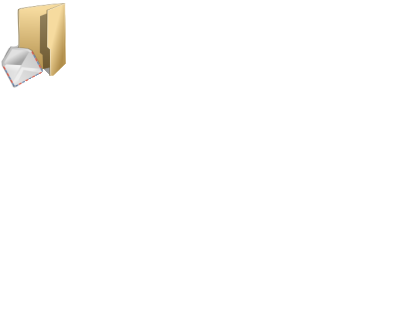
\includegraphics[width=0.95\textwidth]{images/swaml-1.png}}
	  \only<3>{
\includegraphics[width=0.95\textwidth]{images/swaml-2.png}}
	  \only<4>{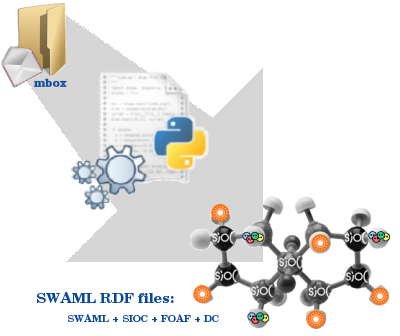
\includegraphics[width=0.95\textwidth]{images/swaml-3.png}}
	\end{center}
   \end{column}
   \begin{column}{0.5\textwidth}
	\begin{Large}batch process:\end{Large}
	\begin{enumerate}
	 \item<2-> mbox
	 \item<3-> parser
	 \item<4-> serialize to RDF/XML 
	\end{enumerate}
   \end{column}
  \end{columns}
}
\frame
{
  \frametitle{SWAML and KML}

  SWAML also generates a KML file that contains the geographical coordinates 
  of the mailing list subscribers.

  \begin{center}
    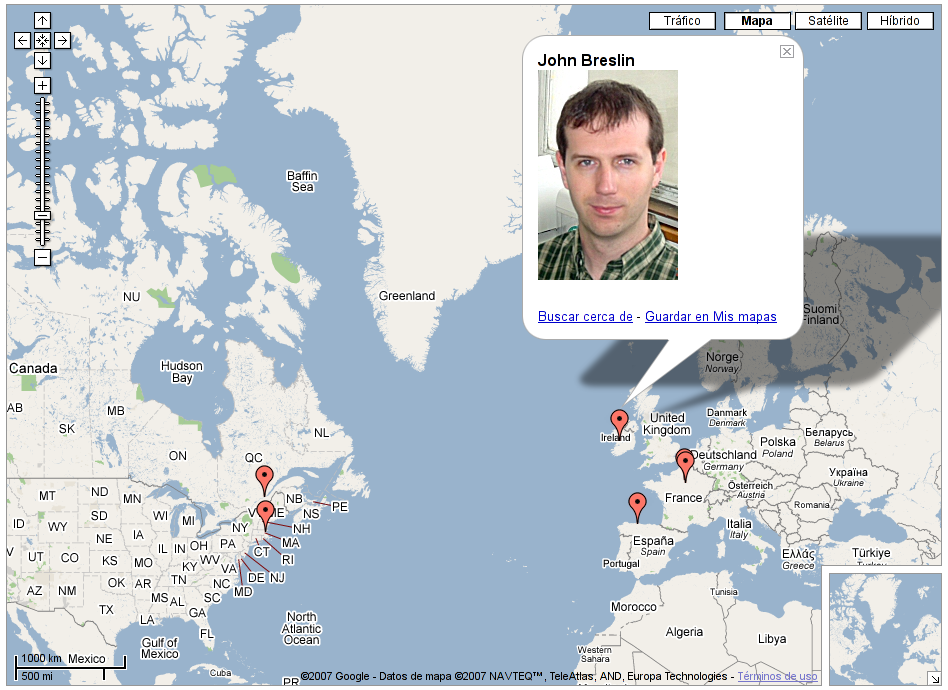
\includegraphics[width=0.7\textwidth]{images/googlemaps.png}
  \end{center}
}
\frame
{
  \frametitle{Buxon}

  \begin{columns}
   \begin{column}{0.32\textwidth}
	\begin{itemize}
	  \item a \texttt{sioc:Forum} browser
	  \item it recomposes mailing lists' threads
	  \item one of the most important implementation of SIOC
	\end{itemize}
   \end{column}
   \begin{column}{0.68\textwidth}
	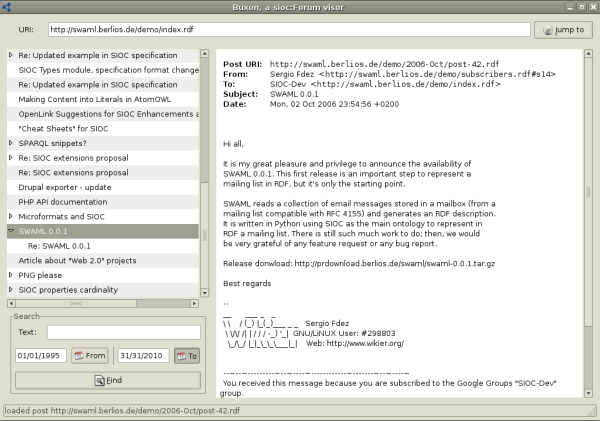
\includegraphics[width=\textwidth]{images/buxon.png}
   \end{column}
  \end{columns}
}

\section{Conclusions and future work}
\frame
{
  \frametitle{Conclusions}

  \begin{Large}
    The SWAML project fulfills a much-needed requirement for the Semantic Web: 
    to be able to refer to semantic versions of e-mail messages and their properties 
    using resource URIs.
  \end{Large}
}
\frame
{
  \frametitle{Future Work}

  \begin{itemize}
   \item \begin{Large}Integration of the SWAML process with popular HTML-based mailing list archivers.\end{Large}
   \item \begin{Large}Integration could be pushed further away through RDFa.\end{Large}
   \item \begin{Large}Semantic annotation relative to the meaning of the messages.\end{Large}
   \item \begin{Large}A simple extension to SWAML that makes it possible to read the contents of a GMail account has 
		been developed.\end{Large}
   \item \begin{Large}SIOC submission to W3C.\end{Large}
  \end{itemize}
}

\section{Demostration}
\frame
{
  \frametitle{Practical demostration}

  \begin{center}
    \LARGE{\textbf{Let's go...}}
  \end{center}
}

\appendix

\section{Acknowledgements}
\frame
{
  \frametitle{Acknowledgements}
  
  \begin{Large}
    The authors would like to express their gratitude to Dr. John Breslin and 
    Uldis Bojars from DERI Galway, whose support and contributions have been 
    of great help to this project. 
  \end{Large}

  \vspace{1cm}

  \begin{Large}
    Also to Ignacio Barrientos by his contribution packaging the project for 
    Debian GNU/Linux.
  \end{Large}
}

\section{More information}
\frame
{
  \begin{center}
    More information at the project Web page:\\
    \vspace{1cm}
    \LARGE{\href{http://swaml.berlios.de/}{http://swaml.berlios.de/}}\\
  \end{center}

}

\section{License}
\frame
{
  \begin{center}
    \LARGE{\textbf{Mailing lists meet\\the Semantic Web}}\\
    \vspace{1cm}
    \vspace{1cm}
    \begin{tiny}
	This talk is distributed under the terms of:\\
	\textbf{CreativeCommons license}\\
	
\includegraphics[width=3.5cm]{images/creativecommons.png}
    \end{tiny}
  \end{center}
}

\end{document}
